\documentclass[10pt]{article}
\usepackage[a4paper,margin=18mm]{geometry}
\usepackage[T1]{fontenc}\usepackage{lmodern}
\usepackage{amsmath,amssymb,booktabs,array,enumitem}
\usepackage{tikz}\usetikzlibrary{shapes.gates.logic.US,positioning,arrows.meta}
\usepackage[hidelinks]{hyperref}
\setlength{\parindent}{0pt}\setlength{\parskip}{4pt}\setlength{\emergencystretch}{2em}
\newcommand{\mos}[4]{\begin{scope}[shift={(#1,#2)}]
\draw(0,.24)--(0,-.24);\draw(0,.2)--(.25,.2)--(.25,.5);\draw(0,-.2)--(.25,-.2)--(.25,-.5);
\draw(-.16,.23)--(-.16,-.23);
\ifnum#4=1\draw(-.26,0)circle(.06);\draw(-.75,0)--(-.32,0);\else\draw(-.75,0)--(-.16,0);\fi
\node[anchor=east,font=\scriptsize]at(-.76,0){$#3$};\end{scope}}
\newcommand{\gnd}[2]{\draw(#1,#2)--(#1,{#2-.12});\draw({#1-.17},{#2-.12})--({#1+.17},{#2-.12});\draw({#1-.11},{#2-.2})--({#1+.11},{#2-.2});}
\newcommand{\rail}[3]{\draw(#1,#2)--(#1,{#2+.14});\node[above,font=\scriptsize]at(#1,{#2+.14}){$#3$};}
% ORIGINAL_LAYOUT_A / ORIGINAL_LAYOUT_B: normalized literal source topology.
% SOLUTION_LAYOUT_A / SOLUTION_LAYOUT_B: labelled MOS schematics, 12 devices each.
% Requires TikZ. No external image, style library, or custom circuit symbol needed.
\newcommand{\VLSIDiff}[2]{\fill[black!17] (#1,-.14) rectangle (#2,.14);\draw (#1,-.14) rectangle (#2,.14);}
\newcommand{\VLSIContact}[2]{\fill (#1-.075,#2-.075) rectangle (#1+.075,#2+.075);}
\newcommand{\VLSIRail}[3]{\draw[line width=3pt,black!35] (#1,#3)--(#2,#3);\draw (#1,#3-.085)--(#2,#3-.085) (#1,#3+.085)--(#2,#3+.085);}
\newcommand{\OriginalLayoutA}{%
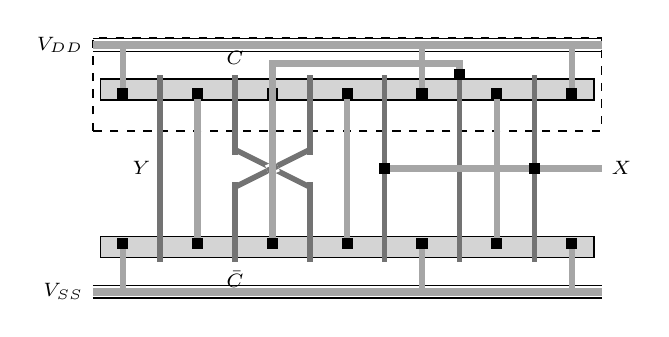
\begin{tikzpicture}[x=.95cm,y=.95cm,font=\scriptsize,line width=.5pt]
\draw[dashed] (-.4,.5) rectangle (6.4,1.75);
\begin{scope}[yshift=1cm]\VLSIDiff{-.3}{6.3}\end{scope}
\begin{scope}[yshift=-1cm]\VLSIDiff{-.3}{6.3}\end{scope}
\VLSIRail{-.4}{6.4}{1.65}\VLSIRail{-.4}{6.4}{-1.65}
\node[left] at (-.4,1.65) {$V_{DD}$};\node[left] at (-.4,-1.65) {$V_{SS}$};
% Six physical columns. Gate 1=Y; gate 2=C/Cbar; gate 3=Cbar/C;
% gate 4=X; gate 5=v; gate 6=X. Split clock gates are not shorted.
\foreach \x in {.5,3.5,4.5,5.5}{\draw[line width=2pt,black!55] (\x,-1.25)--(\x,1.25);}
\foreach \x in {1.5,2.5}{\draw[line width=2pt,black!55] (\x,.18)--(\x,1.25) (\x,-.18)--(\x,-1.25);}
\node[left] at (.5,0) {$Y$};\node[above] at (1.5,1.25) {$C$};\node[below] at (1.5,-1.25) {$\bar C$};
\draw[line width=2pt,black!55] (1.5,-.25)--(2.5,.25);\draw[line width=2pt,black!55] (1.5,.25)--(2.5,-.25);
% Opposite clock routes cross without a contact, shown with a bridge gap.
\draw[white,line width=4pt] (1.93,-.03)--(2.07,.03);\draw[line width=2pt,black!55] (1.93,-.03)--(2.07,.03);
% Supply contacts at physical channel intervals 0, 4, 6.
\foreach \x in {0,4,6}{\draw[line width=2.3pt,black!35] (\x,1)--(\x,1.65) (\x,-1)--(\x,-1.65);\VLSIContact{\x}{1}\VLSIContact{\x}{-1}}
% Inverter output u / transmission node v / feedback output r / X.
\foreach \x in {1,2,3,5}{\draw[line width=2.3pt,black!35] (\x,1)--(\x,-1);\VLSIContact{\x}{1}\VLSIContact{\x}{-1}}
\draw[line width=2.3pt,black!35] (2,.8)--(2,1.4)--(4.5,1.4)--(4.5,1.25);\VLSIContact{4.5}{1.25}
\draw[line width=2.3pt,black!35] (5,0)--(6.4,0) (3.5,0)--(5.5,0);\VLSIContact{3.5}{0}\VLSIContact{5.5}{0}
\node[right] at (6.4,0) {$X$};
\end{tikzpicture}}
\newcommand{\OriginalLayoutB}{%
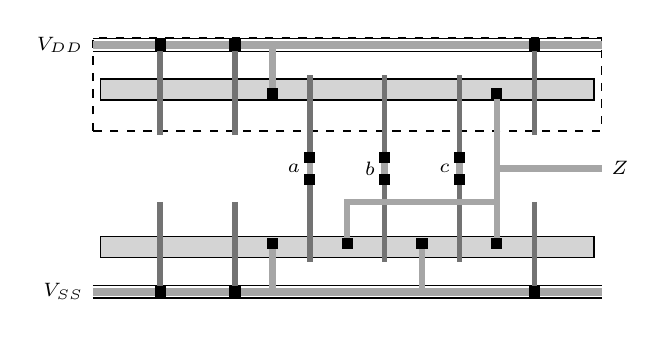
\begin{tikzpicture}[x=.95cm,y=.95cm,font=\scriptsize,line width=.5pt]
\draw[dashed] (-.4,.5) rectangle (6.4,1.75);
\begin{scope}[yshift=1cm]\VLSIDiff{-.3}{6.3}\end{scope}
\begin{scope}[yshift=-1cm]\VLSIDiff{-.3}{6.3}\end{scope}
\VLSIRail{-.4}{6.4}{1.65}\VLSIRail{-.4}{6.4}{-1.65}
\node[left] at (-.4,1.65) {$V_{DD}$};\node[left] at (-.4,-1.65) {$V_{SS}$};
\foreach \x in {.5,1.5,5.5}{\draw[line width=2pt,black!55] (\x,.45)--(\x,1.65) (\x,-.45)--(\x,-1.65);\VLSIContact{\x}{1.65}\VLSIContact{\x}{-1.65}}
\foreach \x/\g in {2.5/a,3.5/b,4.5/c}{\draw[line width=2pt,black!55] (\x,-1.25)--(\x,1.25);\draw[line width=2.3pt,black!35] (\x,-.15)--(\x,.15);\VLSIContact{\x}{-.15}\VLSIContact{\x}{.15}\node[left] at (\x,0) {$\g$};}
\draw[line width=2.3pt,black!35] (2,1)--(2,1.65) (2,-1)--(2,-1.65) (4,-1)--(4,-1.65);
\VLSIContact{2}{1}\VLSIContact{2}{-1}\VLSIContact{4}{-1}
\draw[line width=2.3pt,black!35] (5,1)--(5,-1) (3,-1)--(3,-.45)--(5,-.45);
\VLSIContact{5}{1}\VLSIContact{5}{-1}\VLSIContact{3}{-1}
\draw[line width=2.3pt,black!35] (5,0)--(6.4,0);\node[right] at (6.4,0) {$Z$};
\end{tikzpicture}}

\newcommand{\SolutionLayoutA}{%
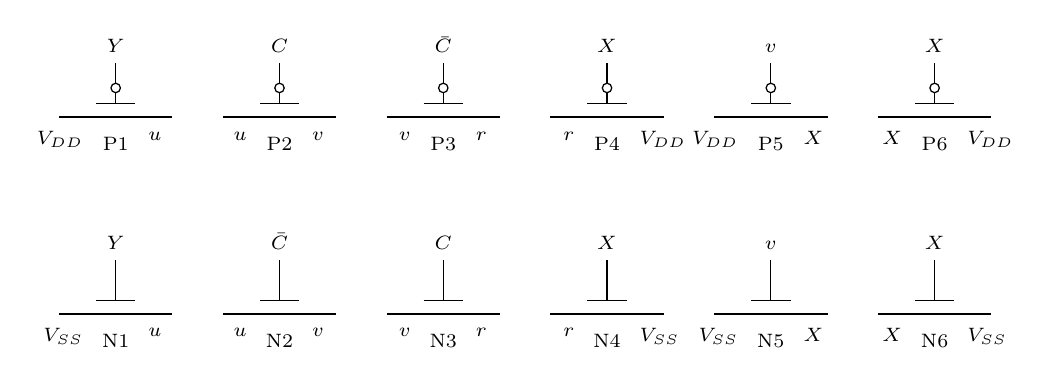
\begin{tikzpicture}[x=1cm,y=1cm,font=\scriptsize,line width=.45pt]
\draw (-0.72,2.5)--(-0.24,2.5) (0.24,2.5)--(0.72,2.5);
\draw[line width=1pt] (-0.24,2.5)--(0.24,2.5);
\draw (-0.25,2.67)--(0.25,2.67);
\draw (0.0,2.67)--(0.0,2.81);\draw (0.0,2.87) circle (.06);\draw (0.0,2.93)--(0.0,3.19);
\node[above] at (0.0,3.19) {$ Y $};
\node[below] at (0.0,2.37) {P1};
\node[anchor=north east] at (-0.29,2.44) {$ V_{DD} $};
\node[anchor=north west] at (0.29,2.44) {$ u $};
\draw (-0.72,0)--(-0.24,0) (0.24,0)--(0.72,0);
\draw[line width=1pt] (-0.24,0)--(0.24,0);
\draw (-0.25,0.17)--(0.25,0.17);
\draw (0.0,0.17)--(0.0,0.69);
\node[above] at (0.0,0.69) {$ Y $};
\node[below] at (0.0,-0.13) {N1};
\node[anchor=north east] at (-0.29,-0.06) {$ V_{SS} $};
\node[anchor=north west] at (0.29,-0.06) {$ u $};
\draw (1.36,2.5)--(1.84,2.5) (2.3200000000000003,2.5)--(2.8,2.5);
\draw[line width=1pt] (1.84,2.5)--(2.3200000000000003,2.5);
\draw (1.83,2.67)--(2.33,2.67);
\draw (2.08,2.67)--(2.08,2.81);\draw (2.08,2.87) circle (.06);\draw (2.08,2.93)--(2.08,3.19);
\node[above] at (2.08,3.19) {$ C $};
\node[below] at (2.08,2.37) {P2};
\node[anchor=north east] at (1.79,2.44) {$ u $};
\node[anchor=north west] at (2.37,2.44) {$ v $};
\draw (1.36,0)--(1.84,0) (2.3200000000000003,0)--(2.8,0);
\draw[line width=1pt] (1.84,0)--(2.3200000000000003,0);
\draw (1.83,0.17)--(2.33,0.17);
\draw (2.08,0.17)--(2.08,0.69);
\node[above] at (2.08,0.69) {$ \bar C $};
\node[below] at (2.08,-0.13) {N2};
\node[anchor=north east] at (1.79,-0.06) {$ u $};
\node[anchor=north west] at (2.37,-0.06) {$ v $};
\draw (3.4400000000000004,2.5)--(3.92,2.5) (4.4,2.5)--(4.88,2.5);
\draw[line width=1pt] (3.92,2.5)--(4.4,2.5);
\draw (3.91,2.67)--(4.41,2.67);
\draw (4.16,2.67)--(4.16,2.81);\draw (4.16,2.87) circle (.06);\draw (4.16,2.93)--(4.16,3.19);
\node[above] at (4.16,3.19) {$ \bar C $};
\node[below] at (4.16,2.37) {P3};
\node[anchor=north east] at (3.87,2.44) {$ v $};
\node[anchor=north west] at (4.45,2.44) {$ r $};
\draw (3.4400000000000004,0)--(3.92,0) (4.4,0)--(4.88,0);
\draw[line width=1pt] (3.92,0)--(4.4,0);
\draw (3.91,0.17)--(4.41,0.17);
\draw (4.16,0.17)--(4.16,0.69);
\node[above] at (4.16,0.69) {$ C $};
\node[below] at (4.16,-0.13) {N3};
\node[anchor=north east] at (3.87,-0.06) {$ v $};
\node[anchor=north west] at (4.45,-0.06) {$ r $};
\draw (5.5200000000000005,2.5)--(6.0,2.5) (6.48,2.5)--(6.96,2.5);
\draw[line width=1pt] (6.0,2.5)--(6.48,2.5);
\draw (5.99,2.67)--(6.49,2.67);
\draw (6.24,2.67)--(6.24,2.81);\draw (6.24,2.87) circle (.06);\draw (6.24,2.93)--(6.24,3.19);
\node[above] at (6.24,3.19) {$ X $};
\node[below] at (6.24,2.37) {P4};
\node[anchor=north east] at (5.95,2.44) {$ r $};
\node[anchor=north west] at (6.53,2.44) {$ V_{DD} $};
\draw (5.5200000000000005,0)--(6.0,0) (6.48,0)--(6.96,0);
\draw[line width=1pt] (6.0,0)--(6.48,0);
\draw (5.99,0.17)--(6.49,0.17);
\draw (6.24,0.17)--(6.24,0.69);
\node[above] at (6.24,0.69) {$ X $};
\node[below] at (6.24,-0.13) {N4};
\node[anchor=north east] at (5.95,-0.06) {$ r $};
\node[anchor=north west] at (6.53,-0.06) {$ V_{SS} $};
\draw (7.6000000000000005,2.5)--(8.08,2.5) (8.56,2.5)--(9.040000000000001,2.5);
\draw[line width=1pt] (8.08,2.5)--(8.56,2.5);
\draw (8.07,2.67)--(8.57,2.67);
\draw (8.32,2.67)--(8.32,2.81);\draw (8.32,2.87) circle (.06);\draw (8.32,2.93)--(8.32,3.19);
\node[above] at (8.32,3.19) {$ v $};
\node[below] at (8.32,2.37) {P5};
\node[anchor=north east] at (8.030000000000001,2.44) {$ V_{DD} $};
\node[anchor=north west] at (8.61,2.44) {$ X $};
\draw (7.6000000000000005,0)--(8.08,0) (8.56,0)--(9.040000000000001,0);
\draw[line width=1pt] (8.08,0)--(8.56,0);
\draw (8.07,0.17)--(8.57,0.17);
\draw (8.32,0.17)--(8.32,0.69);
\node[above] at (8.32,0.69) {$ v $};
\node[below] at (8.32,-0.13) {N5};
\node[anchor=north east] at (8.030000000000001,-0.06) {$ V_{SS} $};
\node[anchor=north west] at (8.61,-0.06) {$ X $};
\draw (9.68,2.5)--(10.16,2.5) (10.64,2.5)--(11.120000000000001,2.5);
\draw[line width=1pt] (10.16,2.5)--(10.64,2.5);
\draw (10.15,2.67)--(10.65,2.67);
\draw (10.4,2.67)--(10.4,2.81);\draw (10.4,2.87) circle (.06);\draw (10.4,2.93)--(10.4,3.19);
\node[above] at (10.4,3.19) {$ X $};
\node[below] at (10.4,2.37) {P6};
\node[anchor=north east] at (10.110000000000001,2.44) {$ X $};
\node[anchor=north west] at (10.69,2.44) {$ V_{DD} $};
\draw (9.68,0)--(10.16,0) (10.64,0)--(11.120000000000001,0);
\draw[line width=1pt] (10.16,0)--(10.64,0);
\draw (10.15,0.17)--(10.65,0.17);
\draw (10.4,0.17)--(10.4,0.69);
\node[above] at (10.4,0.69) {$ X $};
\node[below] at (10.4,-0.13) {N6};
\node[anchor=north east] at (10.110000000000001,-0.06) {$ X $};
\node[anchor=north west] at (10.69,-0.06) {$ V_{SS} $};
\end{tikzpicture}}
\newcommand{\SolutionLayoutB}{%
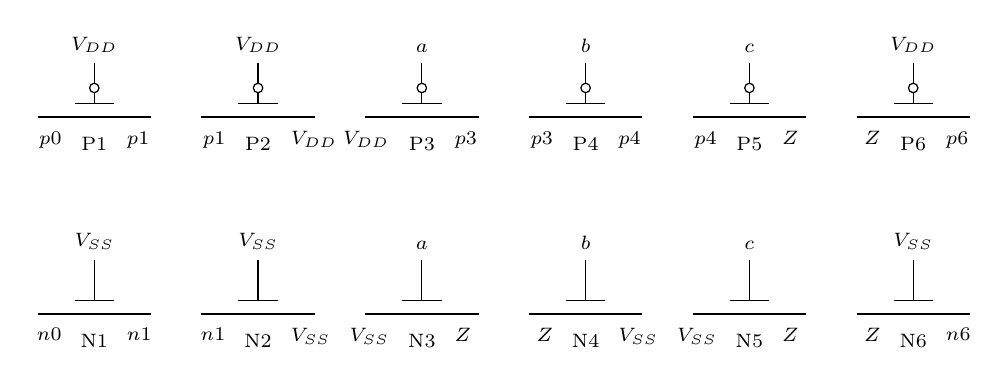
\begin{tikzpicture}[x=1cm,y=1cm,font=\scriptsize,line width=.45pt]
\draw (-0.72,2.5)--(-0.24,2.5) (0.24,2.5)--(0.72,2.5);
\draw[line width=1pt] (-0.24,2.5)--(0.24,2.5);
\draw (-0.25,2.67)--(0.25,2.67);
\draw (0.0,2.67)--(0.0,2.81);\draw (0.0,2.87) circle (.06);\draw (0.0,2.93)--(0.0,3.19);
\node[above] at (0.0,3.19) {$ V_{DD} $};
\node[below] at (0.0,2.37) {P1};
\node[anchor=north east] at (-0.29,2.44) {$ p0 $};
\node[anchor=north west] at (0.29,2.44) {$ p1 $};
\draw (-0.72,0)--(-0.24,0) (0.24,0)--(0.72,0);
\draw[line width=1pt] (-0.24,0)--(0.24,0);
\draw (-0.25,0.17)--(0.25,0.17);
\draw (0.0,0.17)--(0.0,0.69);
\node[above] at (0.0,0.69) {$ V_{SS} $};
\node[below] at (0.0,-0.13) {N1};
\node[anchor=north east] at (-0.29,-0.06) {$ n0 $};
\node[anchor=north west] at (0.29,-0.06) {$ n1 $};
\draw (1.36,2.5)--(1.84,2.5) (2.3200000000000003,2.5)--(2.8,2.5);
\draw[line width=1pt] (1.84,2.5)--(2.3200000000000003,2.5);
\draw (1.83,2.67)--(2.33,2.67);
\draw (2.08,2.67)--(2.08,2.81);\draw (2.08,2.87) circle (.06);\draw (2.08,2.93)--(2.08,3.19);
\node[above] at (2.08,3.19) {$ V_{DD} $};
\node[below] at (2.08,2.37) {P2};
\node[anchor=north east] at (1.79,2.44) {$ p1 $};
\node[anchor=north west] at (2.37,2.44) {$ V_{DD} $};
\draw (1.36,0)--(1.84,0) (2.3200000000000003,0)--(2.8,0);
\draw[line width=1pt] (1.84,0)--(2.3200000000000003,0);
\draw (1.83,0.17)--(2.33,0.17);
\draw (2.08,0.17)--(2.08,0.69);
\node[above] at (2.08,0.69) {$ V_{SS} $};
\node[below] at (2.08,-0.13) {N2};
\node[anchor=north east] at (1.79,-0.06) {$ n1 $};
\node[anchor=north west] at (2.37,-0.06) {$ V_{SS} $};
\draw (3.4400000000000004,2.5)--(3.92,2.5) (4.4,2.5)--(4.88,2.5);
\draw[line width=1pt] (3.92,2.5)--(4.4,2.5);
\draw (3.91,2.67)--(4.41,2.67);
\draw (4.16,2.67)--(4.16,2.81);\draw (4.16,2.87) circle (.06);\draw (4.16,2.93)--(4.16,3.19);
\node[above] at (4.16,3.19) {$ a $};
\node[below] at (4.16,2.37) {P3};
\node[anchor=north east] at (3.87,2.44) {$ V_{DD} $};
\node[anchor=north west] at (4.45,2.44) {$ p3 $};
\draw (3.4400000000000004,0)--(3.92,0) (4.4,0)--(4.88,0);
\draw[line width=1pt] (3.92,0)--(4.4,0);
\draw (3.91,0.17)--(4.41,0.17);
\draw (4.16,0.17)--(4.16,0.69);
\node[above] at (4.16,0.69) {$ a $};
\node[below] at (4.16,-0.13) {N3};
\node[anchor=north east] at (3.87,-0.06) {$ V_{SS} $};
\node[anchor=north west] at (4.45,-0.06) {$ Z $};
\draw (5.5200000000000005,2.5)--(6.0,2.5) (6.48,2.5)--(6.96,2.5);
\draw[line width=1pt] (6.0,2.5)--(6.48,2.5);
\draw (5.99,2.67)--(6.49,2.67);
\draw (6.24,2.67)--(6.24,2.81);\draw (6.24,2.87) circle (.06);\draw (6.24,2.93)--(6.24,3.19);
\node[above] at (6.24,3.19) {$ b $};
\node[below] at (6.24,2.37) {P4};
\node[anchor=north east] at (5.95,2.44) {$ p3 $};
\node[anchor=north west] at (6.53,2.44) {$ p4 $};
\draw (5.5200000000000005,0)--(6.0,0) (6.48,0)--(6.96,0);
\draw[line width=1pt] (6.0,0)--(6.48,0);
\draw (5.99,0.17)--(6.49,0.17);
\draw (6.24,0.17)--(6.24,0.69);
\node[above] at (6.24,0.69) {$ b $};
\node[below] at (6.24,-0.13) {N4};
\node[anchor=north east] at (5.95,-0.06) {$ Z $};
\node[anchor=north west] at (6.53,-0.06) {$ V_{SS} $};
\draw (7.6000000000000005,2.5)--(8.08,2.5) (8.56,2.5)--(9.040000000000001,2.5);
\draw[line width=1pt] (8.08,2.5)--(8.56,2.5);
\draw (8.07,2.67)--(8.57,2.67);
\draw (8.32,2.67)--(8.32,2.81);\draw (8.32,2.87) circle (.06);\draw (8.32,2.93)--(8.32,3.19);
\node[above] at (8.32,3.19) {$ c $};
\node[below] at (8.32,2.37) {P5};
\node[anchor=north east] at (8.030000000000001,2.44) {$ p4 $};
\node[anchor=north west] at (8.61,2.44) {$ Z $};
\draw (7.6000000000000005,0)--(8.08,0) (8.56,0)--(9.040000000000001,0);
\draw[line width=1pt] (8.08,0)--(8.56,0);
\draw (8.07,0.17)--(8.57,0.17);
\draw (8.32,0.17)--(8.32,0.69);
\node[above] at (8.32,0.69) {$ c $};
\node[below] at (8.32,-0.13) {N5};
\node[anchor=north east] at (8.030000000000001,-0.06) {$ V_{SS} $};
\node[anchor=north west] at (8.61,-0.06) {$ Z $};
\draw (9.68,2.5)--(10.16,2.5) (10.64,2.5)--(11.120000000000001,2.5);
\draw[line width=1pt] (10.16,2.5)--(10.64,2.5);
\draw (10.15,2.67)--(10.65,2.67);
\draw (10.4,2.67)--(10.4,2.81);\draw (10.4,2.87) circle (.06);\draw (10.4,2.93)--(10.4,3.19);
\node[above] at (10.4,3.19) {$ V_{DD} $};
\node[below] at (10.4,2.37) {P6};
\node[anchor=north east] at (10.110000000000001,2.44) {$ Z $};
\node[anchor=north west] at (10.69,2.44) {$ p6 $};
\draw (9.68,0)--(10.16,0) (10.64,0)--(11.120000000000001,0);
\draw[line width=1pt] (10.16,0)--(10.64,0);
\draw (10.15,0.17)--(10.65,0.17);
\draw (10.4,0.17)--(10.4,0.69);
\node[above] at (10.4,0.69) {$ V_{SS} $};
\node[below] at (10.4,-0.13) {N6};
\node[anchor=north east] at (10.110000000000001,-0.06) {$ Z $};
\node[anchor=north west] at (10.69,-0.06) {$ n6 $};
\end{tikzpicture}}
\begin{document}
\begin{center}{\Large EE3032 Introduction to VLSI Design---Final}\\Fall 2012\end{center}
Reconstructed from all three supplied original photographs, printed pages 3-1 through 3-3. Original question marks total \textbf{140 points}. Mixed percent/point labels in Q1 are preserved. All figures are editable vector reconstructions that retain the printed circuit connections and qualitative waveforms.\par\medskip
\textbf{1. (40 points)} Answer the following questions.
\begin{enumerate}[label=(\alph*)]
\item Explain the following definitions: (1) physical design, (2) instantiate a cell, and (3) instance. (6\%)
\item List two requirements for drawing the layout of a cell in the cell library. (4 points)
\item List two methods for reducing the power bounce and ground bounce occurring in the IO pads. (4\%)
\item List the major differences among dynamic, domino, and NP-domino logics. (6\%)
\item The dynamic power dissipation (switching power) of a complex gate can be divided into two components. List the two power components. (4 points)
\item List two design rules for avoiding glitch power of a CMOS circuit. (4 points)
\item List two major problems of the dynamic logic. (4 points)
\item List two limitations of the CMOS domino logic. (4 points)
\item What are the core-limited design and pad-limited design? (4 points)
\end{enumerate}\textbf{2. (10 points)} Sketch the Boolean function $f=\overline{A(B+C)+C}$ using each of the following logic design techniques: (1) Dynamic logic (5 points) and (2) Fully differential logic (5 points).\newpage\textbf{3. (15 points)} If an inverter driving a capacitance $C_L$ is operated at $f$ frequency and its supply voltage is $V_{dd}$, then the switching power of the inverter can be expressed as $fC_LV_{dd}^2$. Assume that the $\beta_n$ and $\beta_p$ of the inverter are equal to $\beta$ and an input stimulus with $t_r=t_f=\tau$ is applied, then the short-circuit power of the inverter can be expressed as $k\beta(V_{dd}-V_t)^3\tau f$, where $k$ is a constant. Also, the output $t_r$ and $t_f$ of the inverter can be calculated as $t_r=C_L/(\beta_pV_{dd})$ and $t_f=C_L/(\beta_nV_{dd})$. Complete the following question.

As Figure 1 shows, assume that $\mu_n=2\mu_p$, the gate capacitance of a $W/L$ PMOS or NMOS transistor is $C_g$, $\beta_n$ of a $W/L$ NMOS transistor is $\beta$, and the parasitic capacitance of the drain and wires can be neglected. Let a unit delay be equal to $C_g/(\beta V_{dd})\ ns$. Calculate the dynamic power (switching and short-circuit power) of the inverter chain if the stimulus with frequency $f$ is applied to the inverter chain.\begin{center}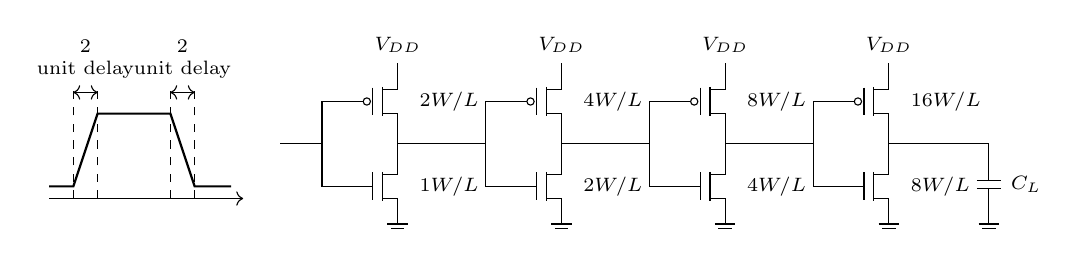
\begin{tikzpicture}[scale=.77,font=\scriptsize]
\begin{scope}[xshift=-5.5cm,yshift=.5cm]
\draw[->](0,0)--(3.2,0);\draw[thick](0,.2)--(.4,.2)--(.8,1.4)--(2,1.4)--(2.4,.2)--(3,.2);
\foreach \x in {.4,.8,2,2.4}{\draw[dashed](\x,0)--(\x,1.9);}
\draw[<->](.4,1.75)--(.8,1.75);\draw[<->](2,1.75)--(2.4,1.75);
\node[above,align=center]at(.6,1.82){2\\unit delay};\node[above,align=center]at(2.2,1.82){2\\unit delay};
\end{scope}
\foreach \x/\pn/\nn in {0/2/1,2.7/4/2,5.4/8/4,8.1/16/8}{
\mos{\x}{2.1}{}{1}\mos{\x}{.7}{}{0}\rail{\x+.25}{2.6}{V_{DD}}\gnd{\x+.25}{.2}
\draw(\x+.25,1.6)--(\x+.25,1.2);\draw(\x-.75,2.1)--(\x-1,2.1)--(\x-1,.7)--(\x-.75,.7);
\node[right]at(\x+.45,2.1){$\pn W/L$};\node[right]at(\x+.45,.7){$\nn W/L$};}
\draw(-1,1.4)--(-1.7,1.4);\draw(.25,1.4)--(1.7,1.4);\draw(2.95,1.4)--(4.4,1.4);\draw(5.65,1.4)--(7.1,1.4);\draw(8.35,1.4)--(10,1.4)--(10,.8);
\draw(9.8,.8)--(10.2,.8);\draw(9.8,.67)--(10.2,.67);\draw(10,.67)--(10,.2);\gnd{10}{.2}\node[right]at(10.2,.73){$C_L$};
\end{tikzpicture}\\Figure 1: An inverter chain driving a $C_L$.\end{center}\textbf{4. (15 points)} Figure 2 shows a dynamic logic gate. Assume that $\mu_n=2\mu_p$, the size $W/L$ of P1 is $4\,\mu m/0.18\,\mu m$, and the channel length of all the transistors is equal to $0.18\,\mu m$. Also, the gate capacitance ($C_g$) of P1 is $C$, i.e., $C_g=C$. Complete the following questions.
\begin{enumerate}[label=(\alph*)]
\item Determine the sizes of the NMOS transistors X1, X2, X3, X4, X5, X6, and N1 such that the rise time and the fall time of the logic gate are equal, i.e., $t_r=t_f$. (5 points)
\item Assume that the gate capacitance of a PMOS or an NMOS is proportional to the gate area of the PMOS or the NMOS. If your boss ask you to design the dynamic gate such that the switching power of the clock (CLK) is smaller than $1.25fCV_{dd}^2$, where $f$ and $V_{dd}$ denote the operation frequency and the power supply of the logic gate, determine the sizes of the NMOS transistors X1, X2, X3, X4, X5, X6, and N1 such that the rise time and the fall time of the logic gate are equal, i.e., $t_r=t_f$. (10 points)
\end{enumerate}\begin{center}\begin{tikzpicture}[scale=.75,font=\small]
\mos{0}{5.1}{CLK}{1}\rail{.25}{5.6}{V_{DD}}\draw(.25,4.6)--(.25,4.1);\fill(.25,4.1)circle(1.5pt);\node[right]at(.45,5.1){P1};
\draw(-1.75,4.1)--(3.25,4.1)node[right]{$Y$};
\mos{-2}{3.4}{X1}{0}\mos{0}{3.4}{X2}{0}\mos{2}{3.4}{X4}{0}\mos{2}{2.1}{X5}{0}\mos{0}{.8}{X3}{0}\mos{2}{.8}{X6}{0}\mos{0}{-.55}{CLK}{0}
\draw(-1.75,4.1)--(-1.75,3.9);\draw(.25,4.1)--(.25,3.9);\draw(2.25,4.1)--(2.25,3.9);\draw(2.25,2.9)--(2.25,2.6);
\draw(.25,2.9)--(.25,1.5)--(2.25,1.5);\draw(2.25,1.6)--(2.25,1.3);\draw(.25,1.5)--(.25,1.3);\fill(.25,1.5)circle(1.5pt);\fill(2.25,1.5)circle(1.5pt);
\draw(-1.75,2.9)--(-1.75,.15)--(2.25,.15);\draw(.25,.3)--(.25,-.05);\draw(2.25,.3)--(2.25,.15);\fill(.25,.15)circle(1.5pt);\gnd{.25}{-1.05}\node[right]at(.45,-.55){N1};
\end{tikzpicture}\\Figure 2: A dynamic logic circuit. X1--X6 label the original nMOS controls.\end{center}\newpage\textbf{5. (15 points)} Figure 3 shows a combinational circuit designed with NP-domino logic. Assume that all the NMOS transistors have the same $\beta_n$ and all the PMOS transistors have the same $\beta_p$, and $\beta_n=\beta_p$. Also, $\mu_n=2\mu_p$ and the gate capacitance of the PMOS and NMOS transistors are $2C$ and $C$, respectively; and the turn-on equivalent resistance of the NMOS transistor or the PMOS transistor is $R$. Complete the following questions.
\begin{enumerate}[label=(\alph*)]
\item Assume that the rise time $t_r$ or fall time $t_f$ of a logic gate can be estimated by the product of the output capacitance of the logic gate and the equivalent resistance of the output charge path or the output discharge path, respectively. Also, the delay $t_d$ of a logic gate can be calculated by $t_d=(t_r+t_f)/2$ and the drain capacitance of the transistors can be neglected. Calculate the contamination delay $t_{cd}$ and the propagation delay $t_{pd}$ of the combinational circuit in terms of $R$ and $C$. (10 points)
\item Assume that the $V_{dd}$ of the combinational circuit is $1.8\,V$ and the threshold voltage of the PMOS transistors is $|V_{tp}|=0.5\,V$. Also, the capacitance of the nodes $x$, $y$, and $z$ are $0.4\,pF$, $0.8\,pF$, and $1.6\,pF$, respectively. Can the combinational circuit be operated correctly? Explain your answer. (5 points)
\end{enumerate}\begin{center}\begin{tikzpicture}[scale=.71,font=\scriptsize]
% Left N-dynamic majority: exactly five data devices plus header/footer.
\mos{0}{3.4}{\phi}{1}\rail{.25}{3.9}{V_{DD}}\draw(.25,2.9)--(.25,2.4);\draw(-1.75,2.4)--(2.25,2.4);\fill(.25,2.4)circle(1.5pt);\node[below]at(.25,2.4){$z$};
\mos{-2}{1.6}{A}{0}\mos{-2}{.2}{B}{0}\draw(-1.75,2.4)--(-1.75,2.1);\draw(-1.75,1.1)--(-1.75,.7);\node[right]at(-1.75,.9){$x$};
\mos{1}{1.6}{C}{0}\draw(1.25,2.4)--(1.25,2.1);\draw(1.25,1.1)--(1.25,.9);\draw(.25,.9)--(2.25,.9);\node[above right]at(1.25,.9){$y$};
\mos{0}{.2}{A}{0}\mos{2}{.2}{B}{0}\draw(.25,.9)--(.25,.7);\draw(2.25,.9)--(2.25,.7);
\draw(-1.75,-.3)--(-1.75,-.6)--(2.25,-.6)--(2.25,-.3);\draw(.25,-.3)--(.25,-1);\fill(.25,-.6)circle(1.5pt);\mos{0}{-1.5}{\phi}{0}\gnd{.25}{-2}
% X: P-clocked inverter, not static CMOS.
\mos{4}{5.6}{\bar\phi}{1}\mos{4}{4.2}{}{1}\mos{4}{2.8}{\bar\phi}{0}\rail{4.25}{6.1}{V_{DD}}\draw(4.25,5.1)--(4.25,4.7);\draw(4.25,3.7)--(4.25,3.3);\gnd{4.25}{2.3}
\draw(.25,2.4)--(2.95,2.4)--(2.95,4.2)--(3.25,4.2);\draw(4.25,3.5)--(6.25,3.5)node[right]{$X$};\fill(4.25,3.5)circle(1.5pt);
% Middle P-dynamic stage: top A/B/C parallel, lower z parallel ABC series.
\mos{8}{3.9}{\bar\phi}{1}\rail{8.25}{4.4}{V_{DD}}\draw(8.25,3.4)--(8.25,3.1);\draw(6.25,3.1)--(10.25,3.1);
\mos{6}{2.4}{A}{1}\mos{8}{2.4}{B}{1}\mos{10}{2.4}{C}{1}
\foreach \x in {6.25,8.25,10.25}{\draw(\x,3.1)--(\x,2.9);\draw(\x,1.9)--(\x,1.6);}
\draw(6.25,1.6)--(10.25,1.6);\fill(8.25,3.1)circle(1.5pt);
\mos{6}{.7}{}{1}\mos{10}{.7}{A}{1}\mos{10}{-.7}{B}{1}\mos{10}{-2.1}{C}{1}
\draw(6.25,1.6)--(6.25,1.2);\draw(10.25,1.6)--(10.25,1.2);\draw(10.25,.2)--(10.25,-.2);\draw(10.25,-1.2)--(10.25,-1.6);
\draw(6.25,.2)--(6.25,-3)--(10.25,-3)--(10.25,-2.6);\draw(8.25,-3)--(8.25,-3.35);\fill(8.25,-3)circle(1.5pt);\mos{8}{-3.85}{\bar\phi}{0}\gnd{8.25}{-4.35}
\draw(2.95,2.4)--(2.95,.7)--(5.25,.7);\fill(2.95,2.4)circle(1.5pt);
% Y: N-clocked inverter. Total device count 7+3+9+3=22.
\mos{13}{-.7}{\phi}{1}\mos{13}{-2.1}{}{0}\mos{13}{-3.5}{\phi}{0}\rail{13.25}{-.2}{V_{DD}}\draw(13.25,-1.2)--(13.25,-1.6);\draw(13.25,-2.6)--(13.25,-3);\gnd{13.25}{-4}
\draw(10.25,-3)--(11.55,-3)--(11.55,-2.1)--(12.25,-2.1);\fill(10.25,-3)circle(1.5pt);\draw(13.25,-1.4)--(14.75,-1.4)node[right]{$Y$};\fill(13.25,-1.4)circle(1.5pt);
\end{tikzpicture}\\Figure 3: A circuit designed with NP-domino logic. The original 22 MOS and all repeated input controls are retained.\end{center}\newpage\textbf{6. (15 points)} Figure 4 shows a sequential circuit. Assume that the clock-to-Q propagation delay ($t_{pcq}$), the clock-to-Q contamination delay ($t_{ccq}$), the setup time ($t_{setup}$), and the hold time ($t_{hold}$) of the registers are $0.4\,ns$, $0.1\,ns$, $0.3\,ns$, and $0.2\,ns$, respectively. Also, the delay of a two-input logic gate (i.e., the XNOR gate, the NOR gate, or the XOR gate) and the inverter is $0.7\,ns$ and $0.3\,ns$, respectively. Complete the following questions.
\begin{enumerate}[label=(\alph*)]
\item If clock skew is $0\,ns$, determine the maximum operation frequency of the sequential circuit. (5 points)
\item If clock skew is $0.5\,ns$, determine the maximum operation frequency of the sequential circuit. (5 points)
\item If the delay of the interconnection between R3 and R4 is $0.05\,ns$ and the clock skew is $0\,ns$, can the circuit be operated correctly? If no, how do you modify the circuit such that it can work correctly? (5 points)
\end{enumerate}\begin{center}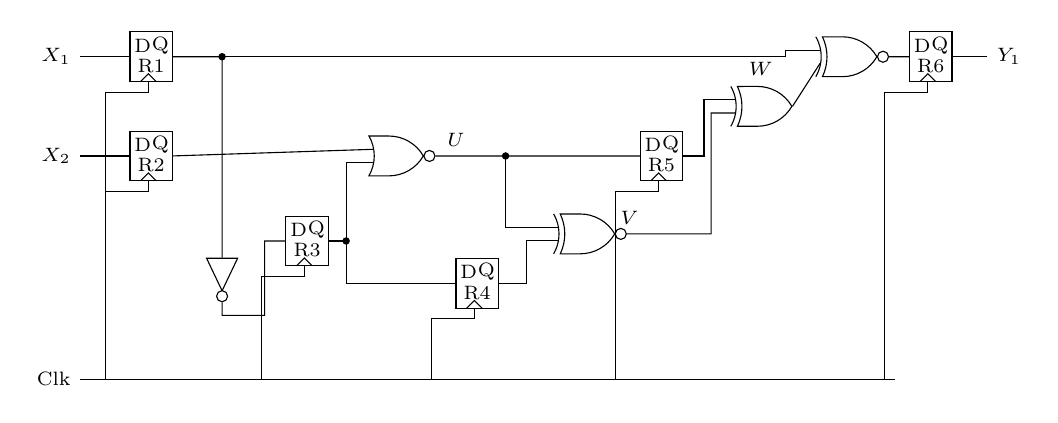
\begin{tikzpicture}[scale=.9,font=\scriptsize]
\draw(-0.3,2.85)rectangle(0.3,3.5500000000000003);\node at(-0.12,3.3600000000000003){D};\node at(0.13,3.3600000000000003){Q};\node at(0,3.0700000000000003){R1};
\draw(-0.15,2.85)--(-0.04,2.96)--(0.07,2.85);
\draw(-0.65,-1.35)--(-0.65,2.7)--(-0.04,2.7)--(-0.04,2.85);
\draw(-0.3,1.4500000000000002)rectangle(0.3,2.15);\node at(-0.12,1.96){D};\node at(0.13,1.96){Q};\node at(0,1.67){R2};
\draw(-0.15,1.4500000000000002)--(-0.04,1.56)--(0.07,1.4500000000000002);
\draw(-0.65,-1.35)--(-0.65,1.3)--(-0.04,1.3)--(-0.04,1.4500000000000002);
\draw(1.9000000000000001,0.25)rectangle(2.5,0.95);\node at(2.08,0.76){D};\node at(2.33,0.76){Q};\node at(2.2,0.47){R3};
\draw(2.0500000000000003,0.25)--(2.16,0.36)--(2.27,0.25);
\draw(1.5500000000000003,-1.35)--(1.5500000000000003,0.09999999999999998)--(2.16,0.09999999999999998)--(2.16,0.25);
\draw(4.3,-0.35)rectangle(4.8999999999999995,0.35);\node at(4.4799999999999995,0.16){D};\node at(4.7299999999999995,0.16){Q};\node at(4.6,-0.13){R4};
\draw(4.449999999999999,-0.35)--(4.56,-0.24)--(4.67,-0.35);
\draw(3.9499999999999997,-1.35)--(3.9499999999999997,-0.5)--(4.56,-0.5)--(4.56,-0.35);
\draw(6.9,1.4500000000000002)rectangle(7.5,2.15);\node at(7.08,1.96){D};\node at(7.33,1.96){Q};\node at(7.2,1.67){R5};
\draw(7.05,1.4500000000000002)--(7.16,1.56)--(7.2700000000000005,1.4500000000000002);
\draw(6.55,-1.35)--(6.55,1.3)--(7.16,1.3)--(7.16,1.4500000000000002);
\draw(10.7,2.85)rectangle(11.3,3.5500000000000003);\node at(10.88,3.3600000000000003){D};\node at(11.13,3.3600000000000003){Q};\node at(11,3.0700000000000003){R6};
\draw(10.85,2.85)--(10.96,2.96)--(11.07,2.85);
\draw(10.35,-1.35)--(10.35,2.7)--(10.96,2.7)--(10.96,2.85);
\draw(-1,-1.35)--(10.5,-1.35);\node[left]at(-1,-1.35){Clk};\draw(-.3,3.2)--(-1,3.2)node[left]{$X_1$};\draw(-.3,1.8)--(-1,1.8)node[left]{$X_2$};\draw(11.3,3.2)--(11.8,3.2)node[right]{$Y_1$};
\node[not gate US,draw,rotate=-90](i)at(1,.2){};\node[nor gate US,draw,logic gate inputs=nn](n)at(3.4,1.8){};
\node[xnor gate US,draw,logic gate inputs=nn](b)at(6.1,.7){};\node[xor gate US,draw,logic gate inputs=nn](m)at(8.6,2.5){};\node[xnor gate US,draw,logic gate inputs=nn](f)at(9.8,3.2){};
\draw(.3,3.2)--(1,3.2)--(i.input);\fill(1,3.2)circle(1.5pt);\draw(1,3.2)--(8.95,3.2)|-(f.input 1);
\draw(.3,1.8)--(n.input 1);\draw(2.5,.6)--(2.75,.6)|-(n.input 2);\fill(2.75,.6)circle(1.5pt);
\draw(n.output)--(5,1.8)--(6.9,1.8);\draw(5,1.8)|-(b.input 1);\fill(5,1.8)circle(1.5pt);\draw(4.9,0)--(5.3,0)|-(b.input 2);\draw(b.output)--(7.9,.7)|-(m.input 2);\draw(7.5,1.8)--(7.8,1.8)|-(m.input 1);\draw(m.output)--(f.input 2);\draw(f.output)--(10.7,3.2);
\node[above]at(4.3,1.8){$U$};\node[above]at(6.75,.7){$V$};\node[above]at(8.6,2.8){$W$};
\draw(i.output)--(1,-.45)--(1.6,-.45)--(1.6,.6)--(1.9,.6);
\draw(2.75,.6)--(2.75,0)--(4.3,0);
\end{tikzpicture}\\Figure 4: A sequential circuit. The middle gate is XOR; the lower and last gates are XNOR.\end{center}\textbf{7. (20 points)} Figure 5 shows two symbolic layouts of two circuits. Draw the transistor-level schematic diagrams of the two circuits.\begin{center}\OriginalLayoutA\quad\OriginalLayoutB\\(a)\hspace{6cm}(b)\\Figure 5: The symbolic layout. Grey horizontal strips are diffusion, light thick routes are Metal 1, dark narrow routes are poly; black squares are contacts. Dashed boxes are n-well. Geometry is normalized while every crossing and connection is retained.\end{center}\newpage\textbf{8. (10 points)} Figure 6 shows the Schmitt CMOS circuit and its voltage transfer curve. Assume that the supply voltage $V_{dd}=1.8\,V$ and the threshold voltage of the NMOS transistors is $V_{tn}=0.6\,V$. If your boss ask you to design the Schmitt CMOS circuit such that its $V_{T+}=1.2\,V$, derive the ratio of $\beta_{N1}$ to $\beta_{N3}$.\begin{center}\begin{tikzpicture}[scale=.91,font=\small]
\mos{0}{3.8}{}{1}\mos{0}{2.4}{}{1}\mos{0}{1}{}{0}\mos{0}{-.4}{}{0}
\rail{.25}{4.3}{V_{dd}}\draw(.25,3.3)--(.25,2.9);\draw(.25,1.9)--(.25,1.5);\draw(.25,.5)--(.25,.1);\gnd{.25}{-.9}
\draw(-.75,3.8)--(-1.25,3.8)--(-1.25,-.4)--(-.75,-.4);\draw(-1.25,2.4)--(-.75,2.4);\draw(-1.25,1)--(-.75,1);\draw(-1.25,1.7)--(-1.8,1.7)node[left]{$V_{in}$};
\node[right]at(.4,3.8){P1};\node[right]at(.4,2.4){P2};\node[right]at(.4,1){N2};\node[right]at(.4,-.4){N1};
\draw(.25,3.1)--(1.15,3.1);\begin{scope}[shift={(1.65,2.85)},rotate=90]\mos{0}{0}{}{1}\end{scope}\draw(2.15,3.1)--(2.5,3.1);\gnd{2.5}{3.1}\node[above]at(1.6,3.28){P3};
\draw(.25,.3)--(1.15,.3);\begin{scope}[shift={(1.65,.55)},rotate=-90]\mos{0}{0}{}{0}\end{scope}\draw(2.15,.3)--(2.5,.3);\rail{2.5}{.3}{V_{dd}}\node[below]at(1.6,-.2){N3};
\draw(.25,1.7)--(3.3,1.7)node[right]{$V_{out}$};\fill(.25,1.7)circle(1.5pt);\draw(1.65,2.1)--(1.65,1.3);\fill(1.65,1.7)circle(1.5pt);
\begin{scope}[xshift=5.5cm]
\draw[->](0,0)--(4.4,0)node[right]{$V_{in}$};\draw[->](0,0)--(0,3.7)node[above]{$V_{out}$};\node[left]at(0,3){$V_{dd}$};
\draw[thick](0,3)--(2.2,3)..controls(2.75,3)and(2.9,2.4)..(2.9,1.4)..controls(2.9,.3)and(3.4,0)..(4,0);
\draw[thick](0,3)--(.5,3)..controls(1.2,3)and(1.4,2.5)..(1.4,1.4)..controls(1.4,.3)and(2.1,0)..(4,0);
\draw[dashed](1.4,0)--(1.4,1.4);\draw[dashed](2.9,0)--(2.9,1.4);\draw[->](1.85,3)--(2.2,3);\draw[->](2.9,2)--(2.9,1.5);\draw[->](1.4,1.5)--(1.4,2);\draw[->](2.2,0)--(1.85,0);
\node[below]at(1.4,0){$V_{T-}$};\node[below]at(2.9,0){$V_{T+}$};\node[below]at(4,0){$V_{dd}$};\node at(1.8,-.9){(b)};\end{scope}\node at(.7,-1.55){(a)};
\end{tikzpicture}\\Figure 6: (a) A CMOS Schmitt circuit. (b) Its voltage transfer curve.\end{center}\end{document}